\documentclass[12pt]{article}

\usepackage{times,fullpage,xspace,fancyhdr,url}
\usepackage[pdftex]{graphicx}
\usepackage[pdftex,
            a4paper,
            colorlinks=true,
            urlcolor=black,
            linkcolor=black,
            citecolor=black,
            bookmarksopen=false,
            bookmarksnumbered=true,
            pdfstartview=FitH]{hyperref}

\usepackage{graphicx}
\usepackage{xspace,color}
\pdfcompresslevel=9
\newcommand{\leaguename}{RoboCup Standard Platform League (NAO) }
\hypersetup{
 pdftitle={\leaguename Technical Challenges 2014},
 pdfauthor={Technical Committee},
}
\usepackage[latin1]{inputenc}
\usepackage{amsmath}
\usepackage{times}

% comment 'disable' in to disable all the todo notes :)
\usepackage
[
%disable
]{todonotes}

\sloppy
\newcommand{\ie}{\mbox{i.\,e.}\xspace}
\newcommand{\eg}{\mbox{e.\,g.}\xspace}
\newcommand{\cf}{\mbox{cf.}\xspace}
\newcommand{\comment}[1]{\marginpar{\pdfannot width 4in height .5in depth 8pt {/Subtype /Text /Contents (#1)}}}
\newcommand{\inparagraph}[1]{\paragraph{#1\hspace{-1em} }}

\long\def\commentk#1{{\bf ++K: #1++}}

% some colors
\definecolor{orange}{rgb}{1,0.5,0}
\definecolor{red}{rgb}{1,0,0}
\definecolor{green}{rgb}{0,1,0}


\title{\leaguename \\ Technical Challenges}
\author{RoboCup Technical Committee}
\date{(2015 technical challenge rules, as of \today)}

\setlength{\parindent}{0pt}
\setlength{\parskip}{6pt plus 6pt minus 3 pt}
\setcounter{tocdepth}{1}
\widowpenalty=10000
\clubpenalty=10000

\pagestyle{fancy}
\lhead{}
\chead{}
\rhead{}
\lfoot{}
\cfoot{}
\rfoot{}

\renewcommand{\headrulewidth}{0.4pt}
\renewcommand{\footrulewidth}{0.4pt}

% needed to align an image and text correctly side by side
\newcommand{\imagebox}[1]{\raisebox{2ex}{\raisebox{-\height}{#1}}}



\begin{document}

\maketitle

At RoboCup 2015, the Standard Platform League will hold three different technical challenges, which are described in this document.

The scores earned in each challenge will vary in magnitude.  Hence, they must be scaled before calculating the overall technical challenge rankings.  Teams who do not participate in a challenge will receive 0 points for that challenge.  The team with the highest total score for a challenge will get 25 points for that challenge, while the team with the lowest total score for a challenge will get 5 points for that challenge.  A linear equation will then be fit to these two points, and each other participating team in that challenge will gain points for that challenge based on this equation.

Questions or comments on these rules should be mailed to {\small \url{rc-spl-tc@lists.robocup.org}}.

\vfill

\renewcommand\contentsname{Challenges}
\tableofcontents
\setcounter{tocdepth}{1}

\thispagestyle{fancy}

\clearpage

\cfoot{\thepage}
\setcounter{page}{1}

\newcommand{\openMinNum}{three}


% % % % % % % % % % % % % % % % % % % % % % % %


\section{Corner Kick Challenge}

describe corner kick challenge

\newpage



% % % % % % % % % % % % % % % % % % % % % % % %



\section{Many Carpets Challenge}
\commentk{I pulled over the proposal from last year, but it should be updates as needed.}
One frequently discussed topic is to exchange the current field carpet for a more challenging surface, \eg artificial lawn.
To assess the current state of the art regarding walking stability and to foster research into this direction, the \textit{Walking Challenge} has been prepared.

In this challenge, a participating robot has to walk over a number of different carpets. The layout of the carpets is depicted in Fig. \ref{fig:walking_challenge}.

\begin{figure}[th!]
\centerline{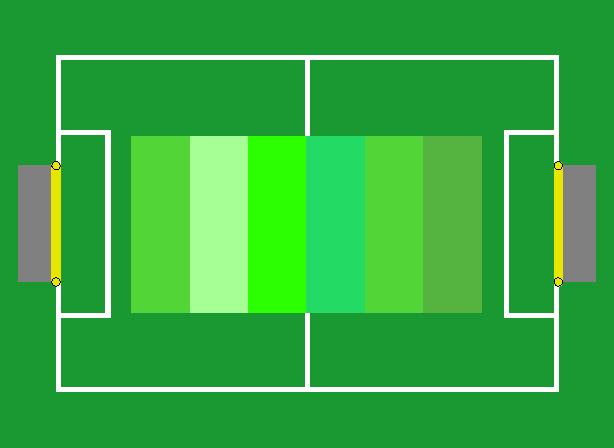
\includegraphics[width=0.6\columnwidth]{figures/walking-challenge}}
\caption{The field layout for the Walking Challenge: Six pieces of different carpets are placed next to each other between the two penalty areas. Each piece of carpet is about 1 meter wide and 3 meters long. A participating robot starts in the center of a penalty area (the team can choose the penalty area), facing the goal on the opposite side of the field.}
\label{fig:walking_challenge}
\end{figure}

For each successfully mastered carpet, the robot can gain either 1, 2, or 4 points: 

\begin{description}
\item[1 point] for successfully traversing a carpet. A carpet is considered as \textit{traversed} if the robot has been completely on the carpet (\ie there has been a point of time at which both feet have been completely on the carpet) and has left it completely afterwards (\ie no part of the robots touches the carpet anymore). Between entering and leaving the carpet, there must be at least three steps. It does not matter if the robot has fallen during traversing the carpet.
\item[2 points] for successfully traversing a carpet and having been standing still for at least 2 seconds while being completely on the carpet. If the robot has fallen while being on the carpet, the 2 points will not be awarded. However, if successfully leaving the carpet, the robot can still achieve 1 point.
\item[4 points] for successfully traversing a carpet and making a full turn of 360 degrees while being completely on the carpet. If the robot has fallen while being on the carpet, the 4 points will not be awarded. However, if successfully leaving the carpet, the robot can still achieve 1 point.
\end{description}

The carpets will be arranged with the most difficult carpets close to the center of the field and the easiest carpets close to the goals. There will not be any gaps between the carpets. However, as the carpets are put on a standard field and are expected to have different heights, teams have to be aware that the overall configuration will contain multiple thresholds over which the robot has to walk.

A robot can only receive one score per carpet. The order of mastered carpets does not matter. The order of performed actions does not matter either. Therefore, it would be possible, for instance, to walk straight over all carpets (and gain 1 point for each carpet) and to return to some of the carpets afterwards to achieve higher scores on these carpets.

Each robot will be given 3 minutes to walk on the field. If a robot falls over and its get up motion fails on a particular surface, the team can request to relocate the robot to one of the starting positions (the team can choose a new starting position for each relocation).

The carpets will be brought to the competition by TC members and the teams. On site, all available carpets will be presented and six carpets will be selected by the TC for the challenge. The selection should cover a broad range of (un)evenness and slippage. Each carpet's difficulty is judged by the TC. All carpets will be green (in any shade) but do not need to be uniform.


\newpage



% % % % % % % % % % % % % % % % % % % % % % % %



\section{Realistic Ball Challenge}

describe the realistic ball challenge


\end{document}

